\documentclass[tikz=true]{standalone}
\usepackage{tikz}
\usepackage{../main/NHQM}

\usetikzlibrary{positioning}
%% helper macros

% The 3D code is based on The drawing is based on Tomas M. Trzeciak's 
% `Stereographic and cylindrical map projections example`: 
% http://www.texample.net/tikz/examples/map-projections/
\newcommand\pgfmathsinandcos[3]{%
  \pgfmathsetmacro#1{sin(#3)}%
  \pgfmathsetmacro#2{cos(#3)}%
}
\newcommand\LongitudePlane[3][current plane]{%
  \pgfmathsinandcos\sinEl\cosEl{#2} % elevation
  \pgfmathsinandcos\sint\cost{#3} % azimuth
  \tikzset{#1/.estyle={cm={\cost,\sint*\sinEl,0,\cosEl,(0,0)}}}
}
\newcommand\LatitudePlane[3][current plane]{%
  \pgfmathsinandcos\sinEl\cosEl{#2} % elevation
  \pgfmathsinandcos\sint\cost{#3} % latitude
  \pgfmathsetmacro\yshift{\cosEl*\sint}
  \tikzset{#1/.estyle={cm={\cost,0,0,\cost*\sinEl,(0,\yshift)}}} %
}
\newcommand\DrawLongitudeCircle[2][1]{
  \LongitudePlane{\angEl}{#2}
  \tikzset{current plane/.prefix style={scale=#1}}
   % angle of "visibility"
  \pgfmathsetmacro\angVis{atan(sin(#2)*cos(\angEl)/sin(\angEl))} %
  \draw[current plane,thin,black] (\angVis:1) arc (\angVis:\angVis+180:1);
  \draw[current plane,thin,dashed] (\angVis-180:1) arc (\angVis-180:\angVis:1);
}%this is fake: for drawing the grid
\newcommand\DrawLongitudeCirclered[2][1]{
  \LongitudePlane{\angEl}{#2}
  \tikzset{current plane/.prefix style={scale=#1}}
   % angle of "visibility"
  \pgfmathsetmacro\angVis{atan(sin(#2)*cos(\angEl)/sin(\angEl))} %
  \draw[current plane,red,thick] (150:1) arc (150:180:1);
  %\draw[current plane,dashed] (-50:1) arc (-50:-35:1);
}%for drawing the grid
\newcommand\DLongredd[2][1]{
  \LongitudePlane{\angEl}{#2}
  \tikzset{current plane/.prefix style={scale=#1}}
   % angle of "visibility"
  \pgfmathsetmacro\angVis{atan(sin(#2)*cos(\angEl)/sin(\angEl))} %
  \draw[current plane,black,dashed, ultra thick] (150:1) arc (150:180:1);
}
\newcommand\DLatred[2][1]{
  \LatitudePlane{\angEl}{#2}
  \tikzset{current plane/.prefix style={scale=#1}}
  \pgfmathsetmacro\sinVis{sin(#2)/cos(#2)*sin(\angEl)/cos(\angEl)}
  % angle of "visibility"
  \pgfmathsetmacro\angVis{asin(min(1,max(\sinVis,-1)))}
  \draw[current plane,dashed,black,ultra thick] (-50:1) arc (-50:-35:1);

}
\newcommand\fillred[2][1]{
  \LongitudePlane{\angEl}{#2}
  \tikzset{current plane/.prefix style={scale=#1}}
   % angle of "visibility"
  \pgfmathsetmacro\angVis{atan(sin(#2)*cos(\angEl)/sin(\angEl))} %
  \draw[current plane,red,thin] (\angVis:1) arc (\angVis:\angVis+180:1);

}

\newcommand\DrawLatitudeCircle[2][1]{
  \LatitudePlane{\angEl}{#2}
  \tikzset{current plane/.prefix style={scale=#1}}
  \pgfmathsetmacro\sinVis{sin(#2)/cos(#2)*sin(\angEl)/cos(\angEl)}
  % angle of "visibility"
  \pgfmathsetmacro\angVis{asin(min(1,max(\sinVis,-1)))}
  \draw[current plane,thin,black] (\angVis:1) arc (\angVis:-\angVis-180:1);
  \draw[current plane,thin,dashed] (180-\angVis:1) arc (180-\angVis:\angVis:1);
}%Defining functions to draw limited latitude circles (for the red mesh)
\newcommand\DrawLatitudeCirclered[2][1]{
  \LatitudePlane{\angEl}{#2}
  \tikzset{current plane/.prefix style={scale=#1}}
  \pgfmathsetmacro\sinVis{sin(#2)/cos(#2)*sin(\angEl)/cos(\angEl)}
  % angle of "visibility"
  \pgfmathsetmacro\angVis{asin(min(1,max(\sinVis,-1)))}
  %\draw[current plane,red,thick] (-\angVis-50:1) arc (-\angVis-50:-\angVis-20:1);
\draw[current plane,red,thick] (-50:1) arc (-50:-35:1);

}


\newcommand\DrawOrbitCircle[2][1]{
  \LatitudePlane{\angEl}{#2}
  \tikzset{current plane/.prefix style={scale=#1}}
  \pgfmathsetmacro\sinVis{sin(#2)/cos(#2)*sin(\angEl)/cos(\angEl)}
  % angle of "visibility"
  \pgfmathsetmacro\angVis{asin(min(1,max(\sinVis,-1)))}
  \draw[current plane,thin,gray] (\angVis:1) arc (\angVis:-\angVis-180:1);
  \draw[current plane,thin,gray] (180-\angVis:1) arc (180-\angVis:\angVis:1);
}


\newcommand\DrawArrowOrbitCircle[2][1]{
  \LatitudePlane{\angEl}{#2}
  \tikzset{current plane/.prefix style={scale=#1}}
  \pgfmathsetmacro\sinVis{sin(#2)/cos(#2)*sin(\angEl)/cos(\angEl)}
  % angle of "visibility"
  \pgfmathsetmacro\angVis{asin(min(1,max(\sinVis,-1)))}
  \draw[current plane,thick,gray, mid arrows] (\angVis:1) arc (\angVis:-\angVis-180:1);
  \draw[current plane,thick,gray, mid arrows] (180-\angVis:1) arc (180-\angVis:\angVis:1);
}


\newcommand\proton[1]{%
\shade[ball color=red] (#1) circle(0.5);
}

\newcommand\neutron[1]{%
\shade[ball color=darkgray] (#1) circle(0.5);
}

\newcommand\blobb[1]{%
\shade[ball color=gray] (#1) circle(0.9);
\shade[ball color=red, opacity =0.15] (#1) circle(0.9);
}

\tikzset{%
  >=latex,
  inner sep=0pt,%
  outer sep=2pt,%
  mark coordinate/.style={inner sep=0pt,outer sep=0pt,minimum size=3pt,
    fill=black,circle}%
}
\usepackage{amsmath}
\usetikzlibrary{arrows}
\pagestyle{empty}
\usepackage{pgfplots}
\usetikzlibrary{calc,fadings,decorations.pathreplacing}

\begin{document}
	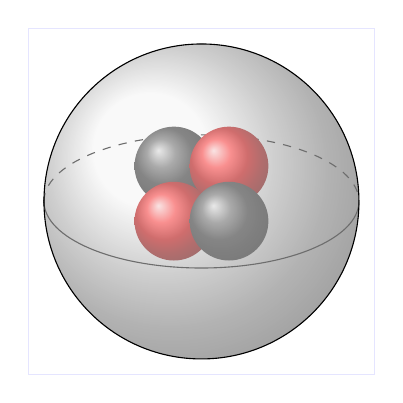
\begin{tikzpicture}[scale=1,every node/.style={minimum size=1cm}]
	%% some definitions
	
	\def\R{2} % sphere radius
	\def\offset{0.1} % sphere radius
	\def\neR{5.25}
	
	\def\angEl{25} % elevation angle
	\def\angAz{-100} % azimuth angle
	\def\angPhiOne{-50} % longitude of point P
	\def\angPhiTwo{-35} % longitude of point Q
	\def\angBeta{30} % latitude of point P and Q
	
	\draw [blue, opacity =0.1] (-2.2,2.2) rectangle (2.2,-2.2);
	
	%% working planes
	
	\pgfmathsetmacro\H{\R*cos(\angEl)} % distance to north pole
	\LongitudePlane[xzplane]{\angEl}{\angAz}
	\LongitudePlane[pzplane]{\angEl}{\angPhiOne}
	\LongitudePlane[qzplane]{\angEl}{\angPhiTwo}
	\LatitudePlane[equator]{\angEl}{0}
	\fill[ball color=white!5] (0,0) circle (\R); % 3D lighting effect
	\coordinate (O) at (0,0);
	% \coordinate[mark coordinate] (N) at (0,\H);
	% \coordinate[mark coordinate] (S) at (0,-\H);
	\path[xzplane] (\R,0) coordinate (XE);
	
    \DrawLatitudeCircle[\R]{0} % equator
	
	
	\neutron{$(-0.35,\offset + 0.35)$}
	\proton{$(0.35,\offset + 0.35)$}
	\proton{$(-0.35,\offset -0.35)$}
	\neutron{$(0.35,\offset -0.35)$}
	
	\draw[fill = gray!10, fill opacity =0.45, ] (0,0) circle (\R);
	    	
\end{tikzpicture}

%%%%%%%%%%%%%%%%%%%%%%%%%%%%%%%%%%%%%%%%%%%%%%%%%%%%%%%%%%%%%%%%%%%%%%%%%%%%%%%%%
\usetikzlibrary{fadings}

	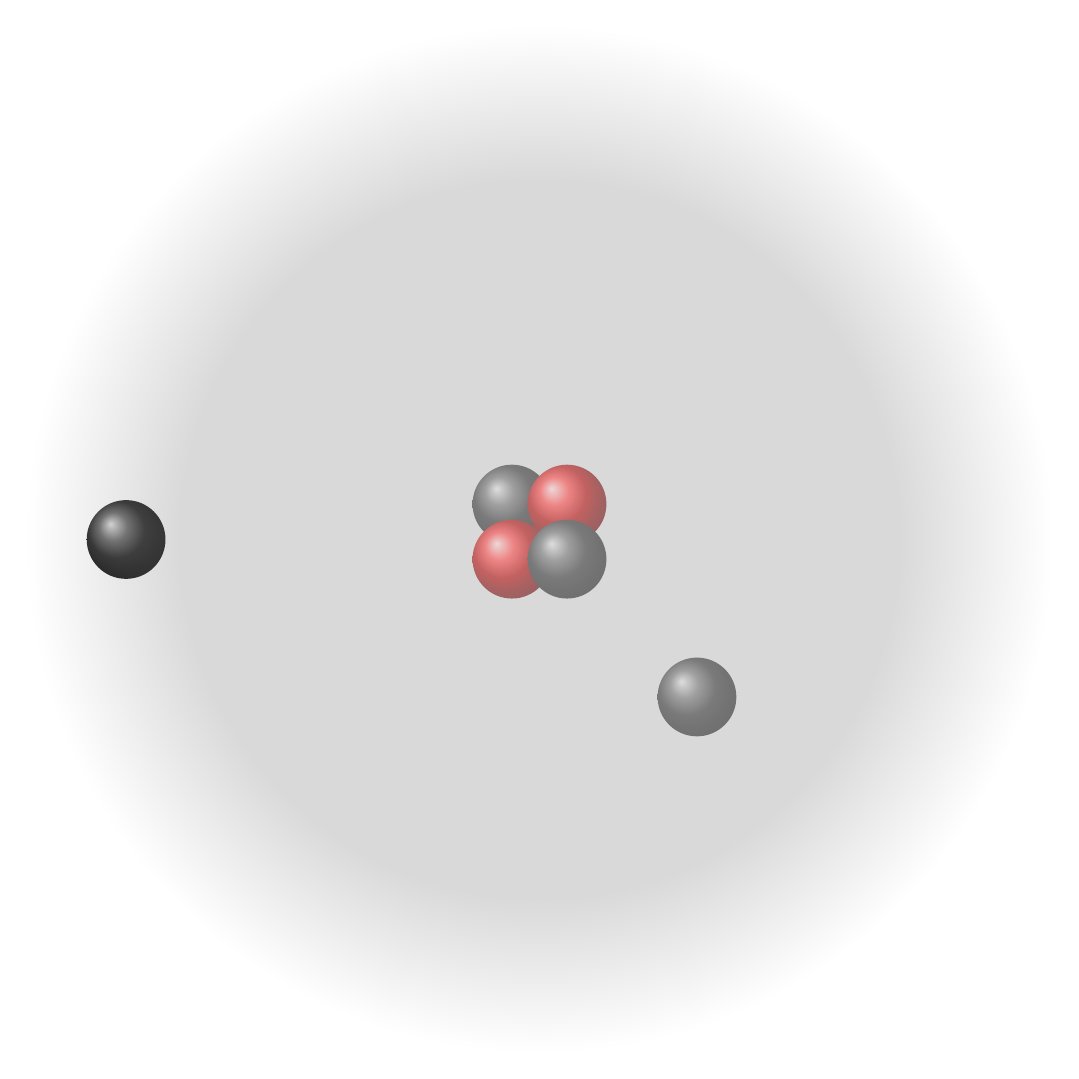
\begin{tikzpicture}[scale=1,every node/.style={minimum size=1cm}]
	%% some definitions
    \tikzfading[name=fade out, inner color=transparent!0, outer color=transparent!100]
	
	
	
	\def\R{2} % sphere radius
	\def\offset{0.1} % sphere radius
	\def\neR{5.25}
	
	
	\neutron{$(-\neR,0)$}
		
		
    \fill [gray, path fading=fade out] (0,0) circle (6.5);
	
	\fill [gray!30, fill opacity =1] (0,0) circle (4.57);

%	\fill[ball color=white!5] (0,0) circle (4.57); % 3D lighting effect
	
	% \fill[color = white!5, opacity = 0.7] (-1.5,1.5) circle (1.25);
% 	\fill[color = white!4, opacity = 0.5] (-1.5,1.5) circle (1.55);
% 	\fill[color = white!3, opacity = 0.3] (-1.5,1.5) circle (1.85);
% 	\fill[color = white!2, opacity = 0.1] (-1.5,1.5) circle (2.25);
	
	\def\angEl{25} % elevation angle
	\def\angAz{-100} % azimuth angle
	\def\angPhiOne{-50} % longitude of point P
	\def\angPhiTwo{-35} % longitude of point Q
	\def\angBeta{30} % latitude of point P and Q
	
	
		
	\neutron{$(-0.35,\offset + 0.35)$}
	\proton{$(0.35,\offset + 0.35)$}
	\proton{$(-0.35,\offset -0.35)$}
	\neutron{$(0.35,\offset -0.35)$}


	\neutron{$(2,-2)$}
	
	\fill[fill = gray!30, fill opacity =0.45, ] (0,0) circle (4.57);
	
	    	
\end{tikzpicture}

%%%%%%%%%%%%%%%%%%%%%%%%%%%%%%%%%%%%%%%%%%%%%%%%%%%%%%%%%%%%%%%%%%%%%%%%%%%%%%%%%

\begin{tikzpicture}
	
	\def\R{2} % sphere radius
	\def\offset{0} % sphere radius

	\def\angEl{25} % elevation angle
	\def\angAz{-100} % azimuth angle
	\def\angPhiOne{-50} % longitude of point P
	\def\angPhiTwo{-35} % longitude of point Q
	\def\angBeta{30} % latitude of point P and Q
	
	\draw [blue, opacity =0] (-3.6,2.5) rectangle (3.2,-2.5);
	
	
	\neutron{$(-0.35,\offset + 0.35)$}
	\proton{$(0.35,\offset + 0.35)$}
	\proton{$(-0.35,\offset -0.35)$}
	\neutron{$(0.35,\offset -0.35)$}


    \DrawArrowOrbitCircle[3]{0} % equator
	
	\draw[thick, mid arrows, gray] (3,-2) -- (-1.25,-1.156);
	\draw[thick, mid arrows, gray] (-1.25,1.156) -- (3,2);

		
	\neutron{$(-3,0)$}
		
\end{tikzpicture}

%%%%%%%%%%%%%%%%%%%%%%%%%%%%%%%%%%%%%%%%%%%%%%%%%%%%%%%%%%%%%%%%%%%%%%%%%%%%%%%%%
 \usetikzlibrary{snakes}
\begin{tikzpicture}
	
	\def\R{2} % sphere radius
	\def\offset{0} % sphere radius

	\def\angEl{25} % elevation angle
	\def\angAz{-100} % azimuth angle
	\def\angPhiOne{-50} % longitude of point P
	\def\angPhiTwo{-35} % longitude of point Q
	\def\angBeta{30} % latitude of point P and Q
	
	
	\draw [blue, opacity =0] (-3.6,2.5) rectangle (3.2,-2.5);
	
	\blobb{0,0}
	\begin{scope}[<->, decoration={snake, post length=3mm, pre length=3mm}, gray, thick]
		 \draw[decorate, thick] (-2.4,0) -- (-1.05,0);
	\end{scope}
	
	

    \DrawArrowOrbitCircle[3]{0} % equator
	
	\draw[thick, mid arrows, gray] (3,-2) -- (-1.25,-1.156);
	\draw[thick, mid arrows, gray] (-1.25,1.156) -- (3,2);
	
	\neutron{$(-3,0)$}
		
\end{tikzpicture}

%%%%%%%%%%%%%%%%%%%%%%%%%%%%%%%%%%%%%%%%%%%%%%%%%%%%%%%%%%%%%%%%%%%%%%%%%%%%%%%%%
\usetikzlibrary{fadings}

	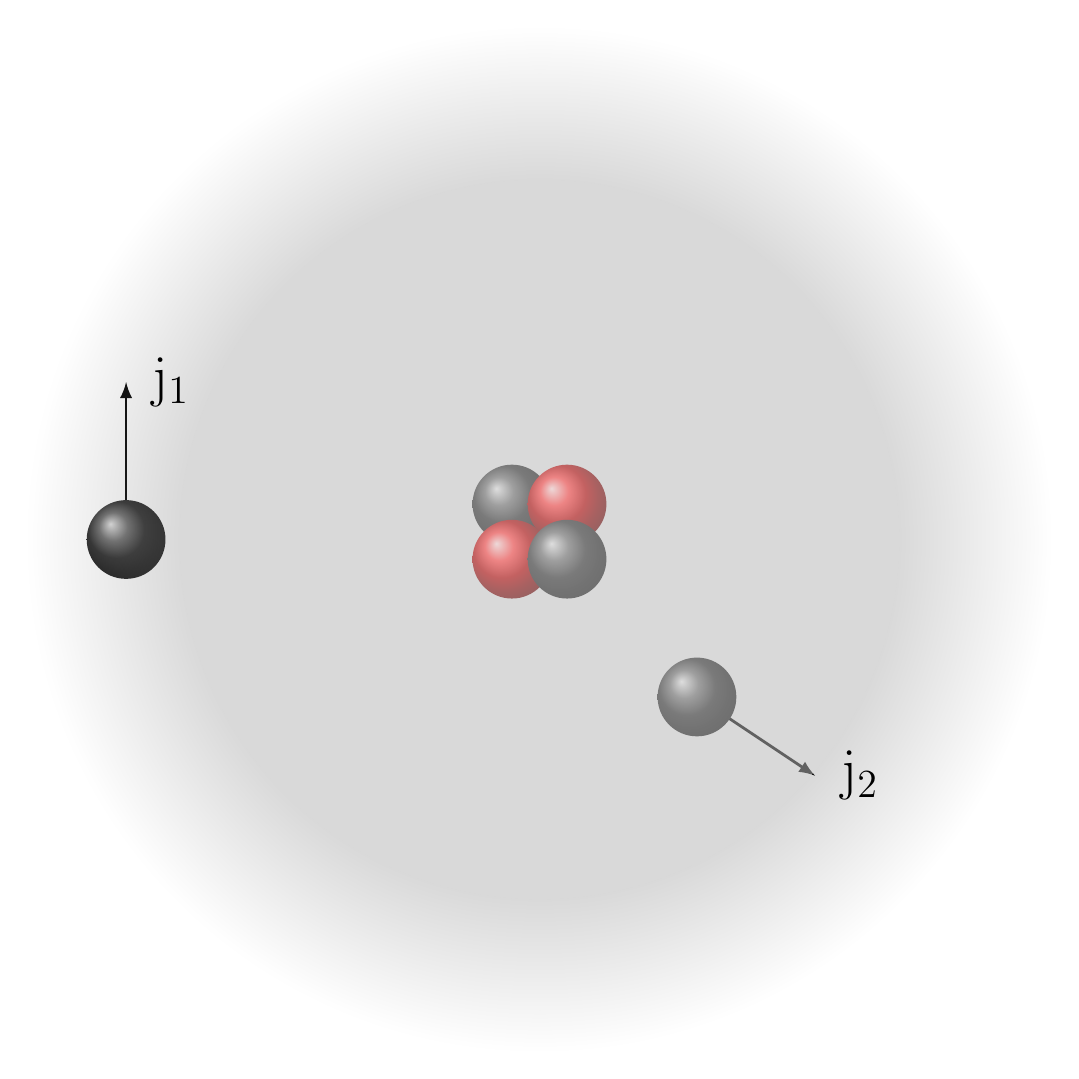
\begin{tikzpicture}[scale=1,every node/.style={minimum size=1cm}]
	%% some definitions
    \tikzfading[name=fade out, inner color=transparent!0, outer color=transparent!100]
	
	
	
	\def\R{2} % sphere radius
	\def\offset{0.1} % sphere radius
	\def\neR{5.25}
	

	\draw[arrows=->,line width=1pt](-\neR,0)--(-\neR,2);
	
	\neutron{$(-\neR,0)$}
		
		
    \fill [gray, path fading=fade out] (0,0) circle (6.5);
	
	\fill [gray!30, fill opacity =1] (0,0) circle (4.57);
	\draw[arrows=->,line width=1pt](2,-2)--(3.5,-3);
%	\fill[ball color=white!5] (0,0) circle (4.57); % 3D lighting effect
	
	% \fill[color = white!5, opacity = 0.7] (-1.5,1.5) circle (1.25);
% 	\fill[color = white!4, opacity = 0.5] (-1.5,1.5) circle (1.55);
% 	\fill[color = white!3, opacity = 0.3] (-1.5,1.5) circle (1.85);
% 	\fill[color = white!2, opacity = 0.1] (-1.5,1.5) circle (2.25);
	
	\def\angEl{25} % elevation angle
	\def\angAz{-100} % azimuth angle
	\def\angPhiOne{-50} % longitude of point P
	\def\angPhiTwo{-35} % longitude of point Q
	\def\angBeta{30} % latitude of point P and Q
	
	
		
	\neutron{$(-0.35,\offset + 0.35)$}
	\proton{$(0.35,\offset + 0.35)$}
	\proton{$(-0.35,\offset -0.35)$}
	\neutron{$(0.35,\offset -0.35)$}


	\neutron{$(2,-2)$}
	
	\fill[fill = gray!30, fill opacity =0.45, ] (0,0) circle (4.57);
	\node[above,right,font=\huge] (why1) at (-\neR,2) {j$_1$};
	\node[above,right,font=\huge] (why1) at (3.5,-3) {j$_2$};
\end{tikzpicture}

%%%%%%%%%%%%%%%%%%%%%%%%%%%%%%%%%%%%%%%%%%%%%%%%%%%%%%%%%%%%%%%%%%%%%%%%%%%%%%%%%
\usetikzlibrary{fadings}

	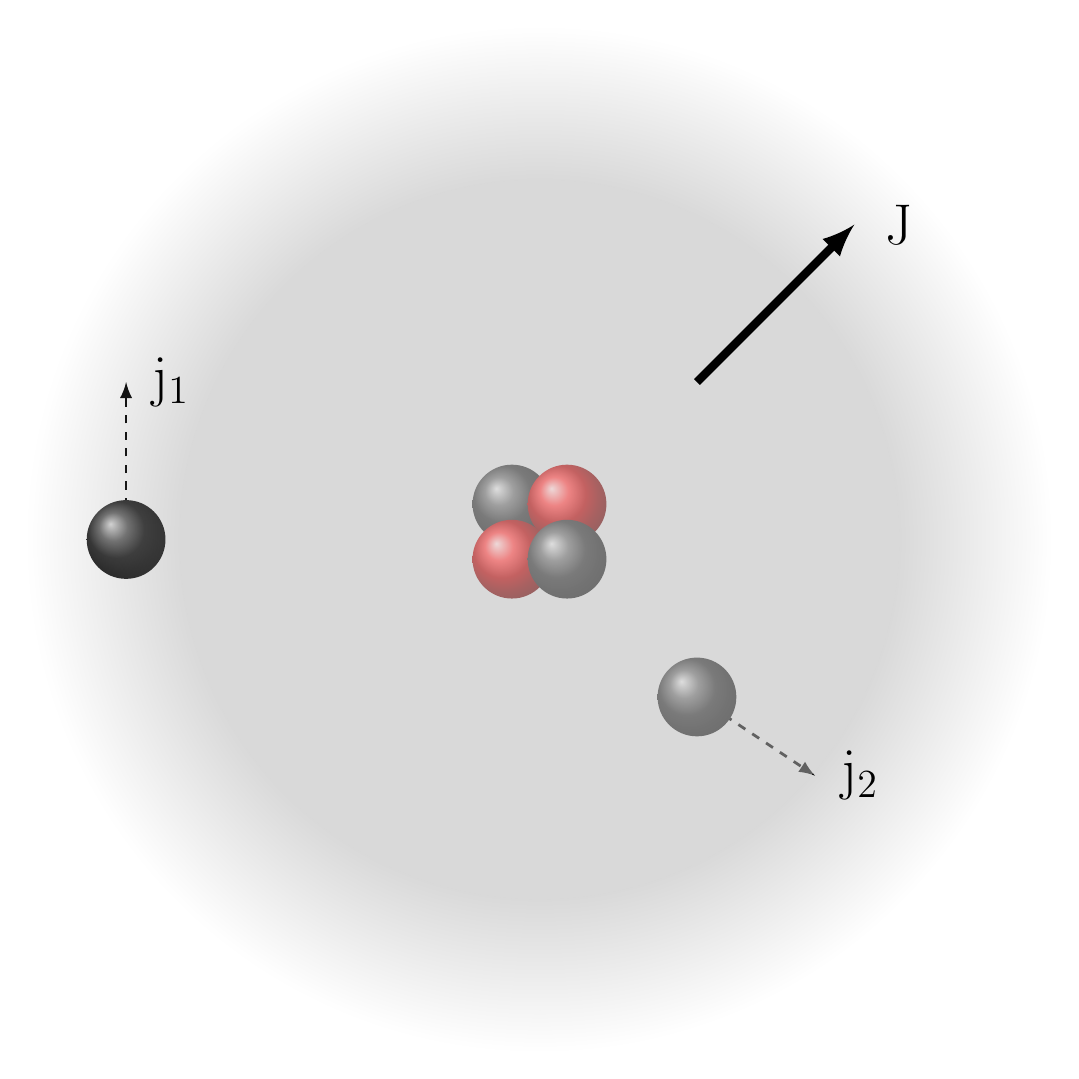
\begin{tikzpicture}[scale=1,every node/.style={minimum size=1cm}]
	%% some definitions
    \tikzfading[name=fade out, inner color=transparent!0, outer color=transparent!100]
	
	
	
	\def\R{2} % sphere radius
	\def\offset{0.1} % sphere radius
	\def\neR{5.25}
	
	\draw[arrows=->,line width=1pt,dashed](-\neR,0)--(-\neR,2);	
	\neutron{$(-\neR,0)$}
		
		
    \fill [gray, path fading=fade out] (0,0) circle (6.5);
	
	\fill [gray!30, fill opacity =1] (0,0) circle (4.57);

%	\fill[ball color=white!5] (0,0) circle (4.57); % 3D lighting effect
	
	% \fill[color = white!5, opacity = 0.7] (-1.5,1.5) circle (1.25);
% 	\fill[color = white!4, opacity = 0.5] (-1.5,1.5) circle (1.55);
% 	\fill[color = white!3, opacity = 0.3] (-1.5,1.5) circle (1.85);
% 	\fill[color = white!2, opacity = 0.1] (-1.5,1.5) circle (2.25);
	\draw[arrows=->,line width=1pt,dashed](2,-2)--(3.5,-3);	
	\def\angEl{25} % elevation angle
	\def\angAz{-100} % azimuth angle
	\def\angPhiOne{-50} % longitude of point P
	\def\angPhiTwo{-35} % longitude of point Q
	\def\angBeta{30} % latitude of point P and Q
	
	
		
	\neutron{$(-0.35,\offset + 0.35)$}
	\proton{$(0.35,\offset + 0.35)$}
	\proton{$(-0.35,\offset -0.35)$}
	\neutron{$(0.35,\offset -0.35)$}


	\neutron{$(2,-2)$}


	\fill[fill = gray!30, fill opacity =0.45, ] (0,0) circle (4.57);
	\draw[arrows=->,line width=3pt](2,2)--(4,4);
	\node[above,right,font=\huge] (why1) at (4,4) {J};
	\node[above,right,font=\huge] (why1) at (-\neR,2) {j$_1$};
	\node[above,right,font=\huge] (why1) at (3.5,-3) {j$_2$};
	
%	\draw[level] at (3,3) node[none]{J};

	
\end{tikzpicture}

%%%%%%%%%%%%%%%%%%%%%%%%%%%%%%%%%%%%%%%%%%%%%%%%%%%%%%%%%%%%%%%%%%%%%%%%%%%%%%%%%
\usetikzlibrary{fadings}

	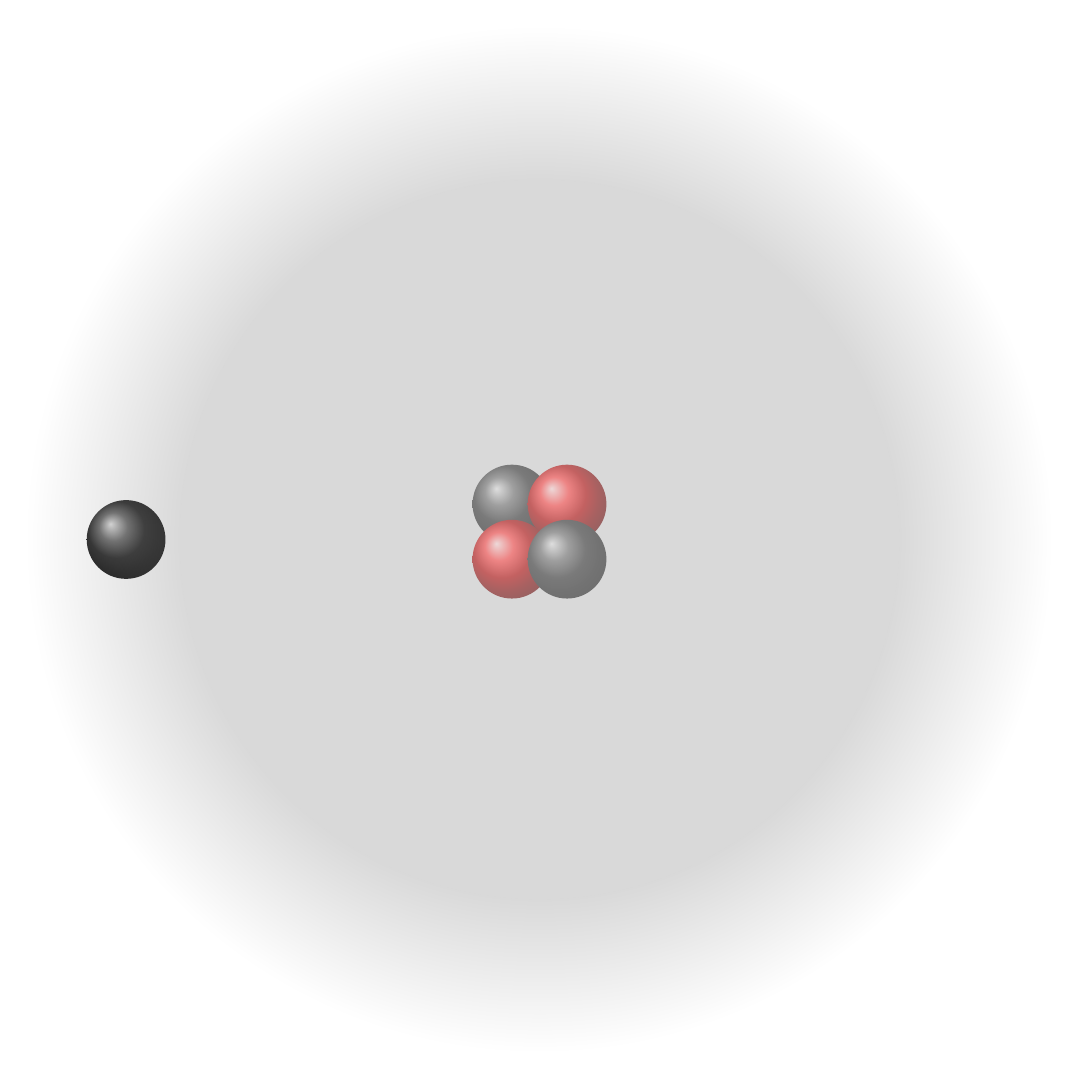
\begin{tikzpicture}[scale=1,every node/.style={minimum size=1cm}]
	%% some definitions
    \tikzfading[name=fade out, inner color=transparent!0, outer color=transparent!100]
	
	
	
	\def\R{2} % sphere radius
	\def\offset{0.1} % sphere radius
	\def\neR{5.25}
	
	
	\neutron{$(-\neR,0)$}
		
		
    \fill [gray, path fading=fade out] (0,0) circle (6.5);
	
	\fill [gray!30, fill opacity =1] (0,0) circle (4.57);

%	\fill[ball color=white!5] (0,0) circle (4.57); % 3D lighting effect
	
	% \fill[color = white!5, opacity = 0.7] (-1.5,1.5) circle (1.25);
% 	\fill[color = white!4, opacity = 0.5] (-1.5,1.5) circle (1.55);
% 	\fill[color = white!3, opacity = 0.3] (-1.5,1.5) circle (1.85);
% 	\fill[color = white!2, opacity = 0.1] (-1.5,1.5) circle (2.25);
	
	\def\angEl{25} % elevation angle
	\def\angAz{-100} % azimuth angle
	\def\angPhiOne{-50} % longitude of point P
	\def\angPhiTwo{-35} % longitude of point Q
	\def\angBeta{30} % latitude of point P and Q
	
	
		
	\neutron{$(-0.35,\offset + 0.35)$}
	\proton{$(0.35,\offset + 0.35)$}
	\proton{$(-0.35,\offset -0.35)$}
	\neutron{$(0.35,\offset -0.35)$}


%	\neutron{$(2,-2)$}
	
	\fill[fill = gray!30, fill opacity =0.45, ] (0,0) circle (4.57);
	
	    	
\end{tikzpicture}

%%%%%%%%%%%%%%%%%%%%%%%%%%%%%%%%%%%%%%%%%%%%%%%%%%%%%%%%%%%%%%%%%%%%%%%%%%%%%%%%%
\usetikzlibrary{fadings}

	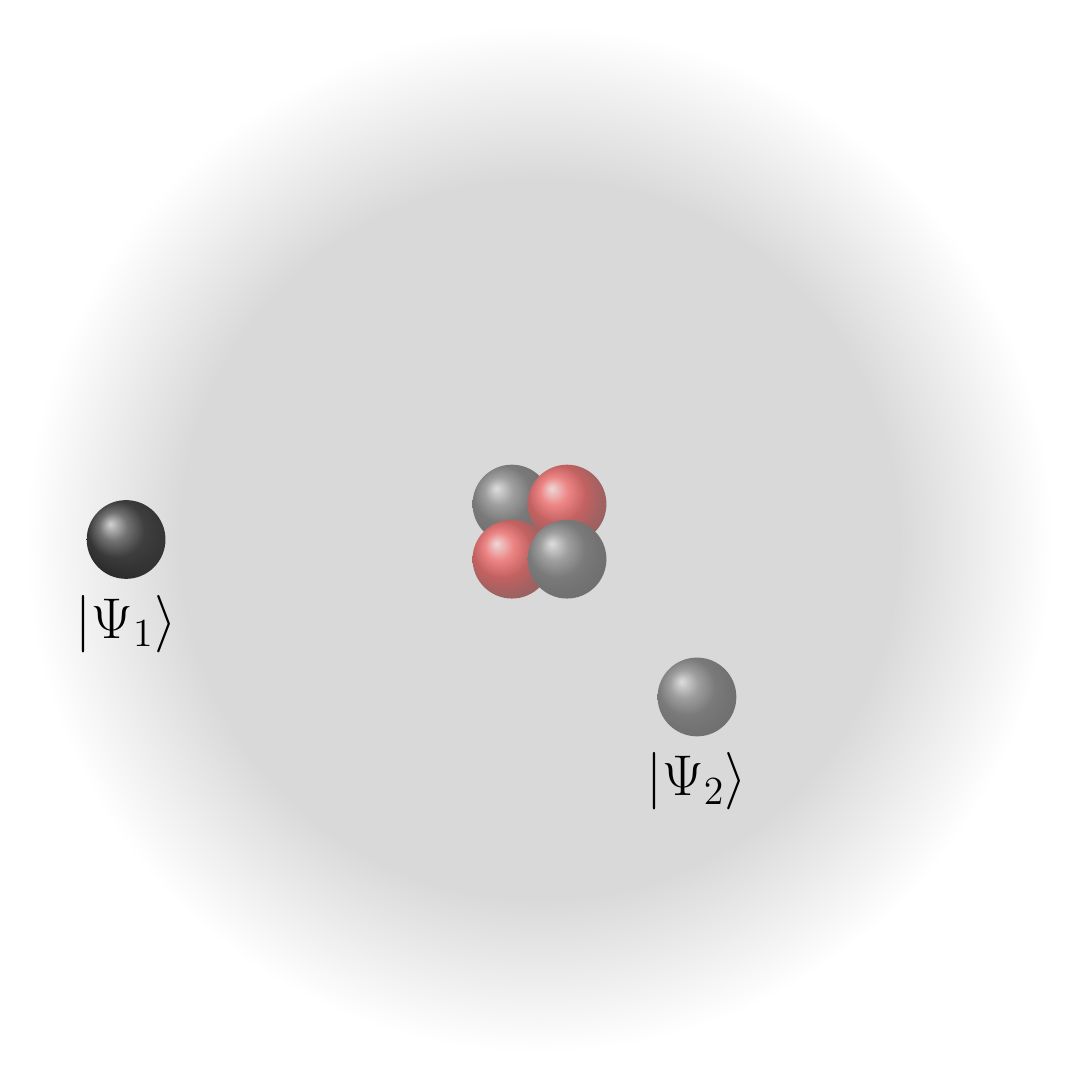
\begin{tikzpicture}[scale=1,every node/.style={minimum size=1cm}]
	%% some definitions
    \tikzfading[name=fade out, inner color=transparent!0, outer color=transparent!100]
	
	
	
	\def\R{2} % sphere radius
	\def\offset{0.1} % sphere radius
	\def\neR{5.25}
	
	
	\neutron{$(-\neR,0)$}
		
		
    \fill [gray, path fading=fade out] (0,0) circle (6.5);
	
	\fill [gray!30, fill opacity =1] (0,0) circle (4.57);

%	\fill[ball color=white!5] (0,0) circle (4.57); % 3D lighting effect
	
	% \fill[color = white!5, opacity = 0.7] (-1.5,1.5) circle (1.25);
% 	\fill[color = white!4, opacity = 0.5] (-1.5,1.5) circle (1.55);
% 	\fill[color = white!3, opacity = 0.3] (-1.5,1.5) circle (1.85);
% 	\fill[color = white!2, opacity = 0.1] (-1.5,1.5) circle (2.25);
	
	\def\angEl{25} % elevation angle
	\def\angAz{-100} % azimuth angle
	\def\angPhiOne{-50} % longitude of point P
	\def\angPhiTwo{-35} % longitude of point Q
	\def\angBeta{30} % latitude of point P and Q
	
	
		
	\neutron{$(-0.35,\offset + 0.35)$}
	\proton{$(0.35,\offset + 0.35)$}
	\proton{$(-0.35,\offset -0.35)$}
	\neutron{$(0.35,\offset -0.35)$}


	\neutron{$(2,-2)$}
	
	\fill[fill = gray!30, fill opacity =0.45, ] (0,0) circle (4.57);
	
	\node[below,font=\huge] (why1) at (-\neR,-0.5) {$|\Psi_1\rangle$};
	\node[below,font=\huge] (why1) at (2,-2.5) {$|\Psi_2\rangle$};
	
	    	
\end{tikzpicture}


\end{document} 